% Chapter 2

\chapter{Electrocardiography overview}
\label{Chapter2} 

This chapter will introduce some basic but fundamental concepts about electrocardiography starting from the heart to the ECG and all issues related to the topic. We will start introducing the heart, its functionality and the entire circulatory system.\\
After that we will describe in details the electrical activity inside the heart and how heart beats are generated. Following there will be a description of the electrocardiogram and the ECG signals. In the last section of this chapter we will discuss about all the noises and interference related to the ECG signal during its acquisition. 

\section{The heart}
\label{TheHeart}
This chapter’s focus is to describe in details the human heart. We will start from the structure to end up describing the heart functionality.

\subsection{Human heart structure}
The human heart is an organ that pumps blood throughout the body via the circulatory system, supplying oxygen and nutrients to the tissues and removing carbon dioxide and other wastes.\\
This fundamental organ has four chambers: two upper chambers(the atrial) and two lower ones(the ventricles). The right atrium and the right ventricle together make up the “right heart”, and the left atrium and left ventricle make up the”left heart”. The two sides of the heart are separated by a muscle called the septum. \\
A double-walled sac called the pericardium, encases the heart, which serves to protect the heart and anchors it inside the chest. Between the outer layer, the parietal pericardium, and the inner layer, the serous pericardium, runs pericardial fluid, which lubricates the heart during contractions and movements of the lungs and diaphragm.
The heart outer wall consists of three layers. The outermost wall layer, or epicardium, is the inner wall of the pericardium.  The middle layer, or myocardium, contains the muscle that contracts. The inner layer, or endocardium, is the lining that contacts the blood.\\
The tricuspid valve and the mitral valve make up the atrioventricular (AV) valves, which connect the atria and the ventricles. The pulmonary semilunar valve separates the right ventricle from the pulmonary artery, and the aortic valve separates the left ventricle from the aorta. The heartstrings, or chordae tendineae, anchor the valves to heart muscles.\\
The sinoatrial node produces the electrical pulses that drive heart contractions.
\begin{figure}[ht!]
\centering
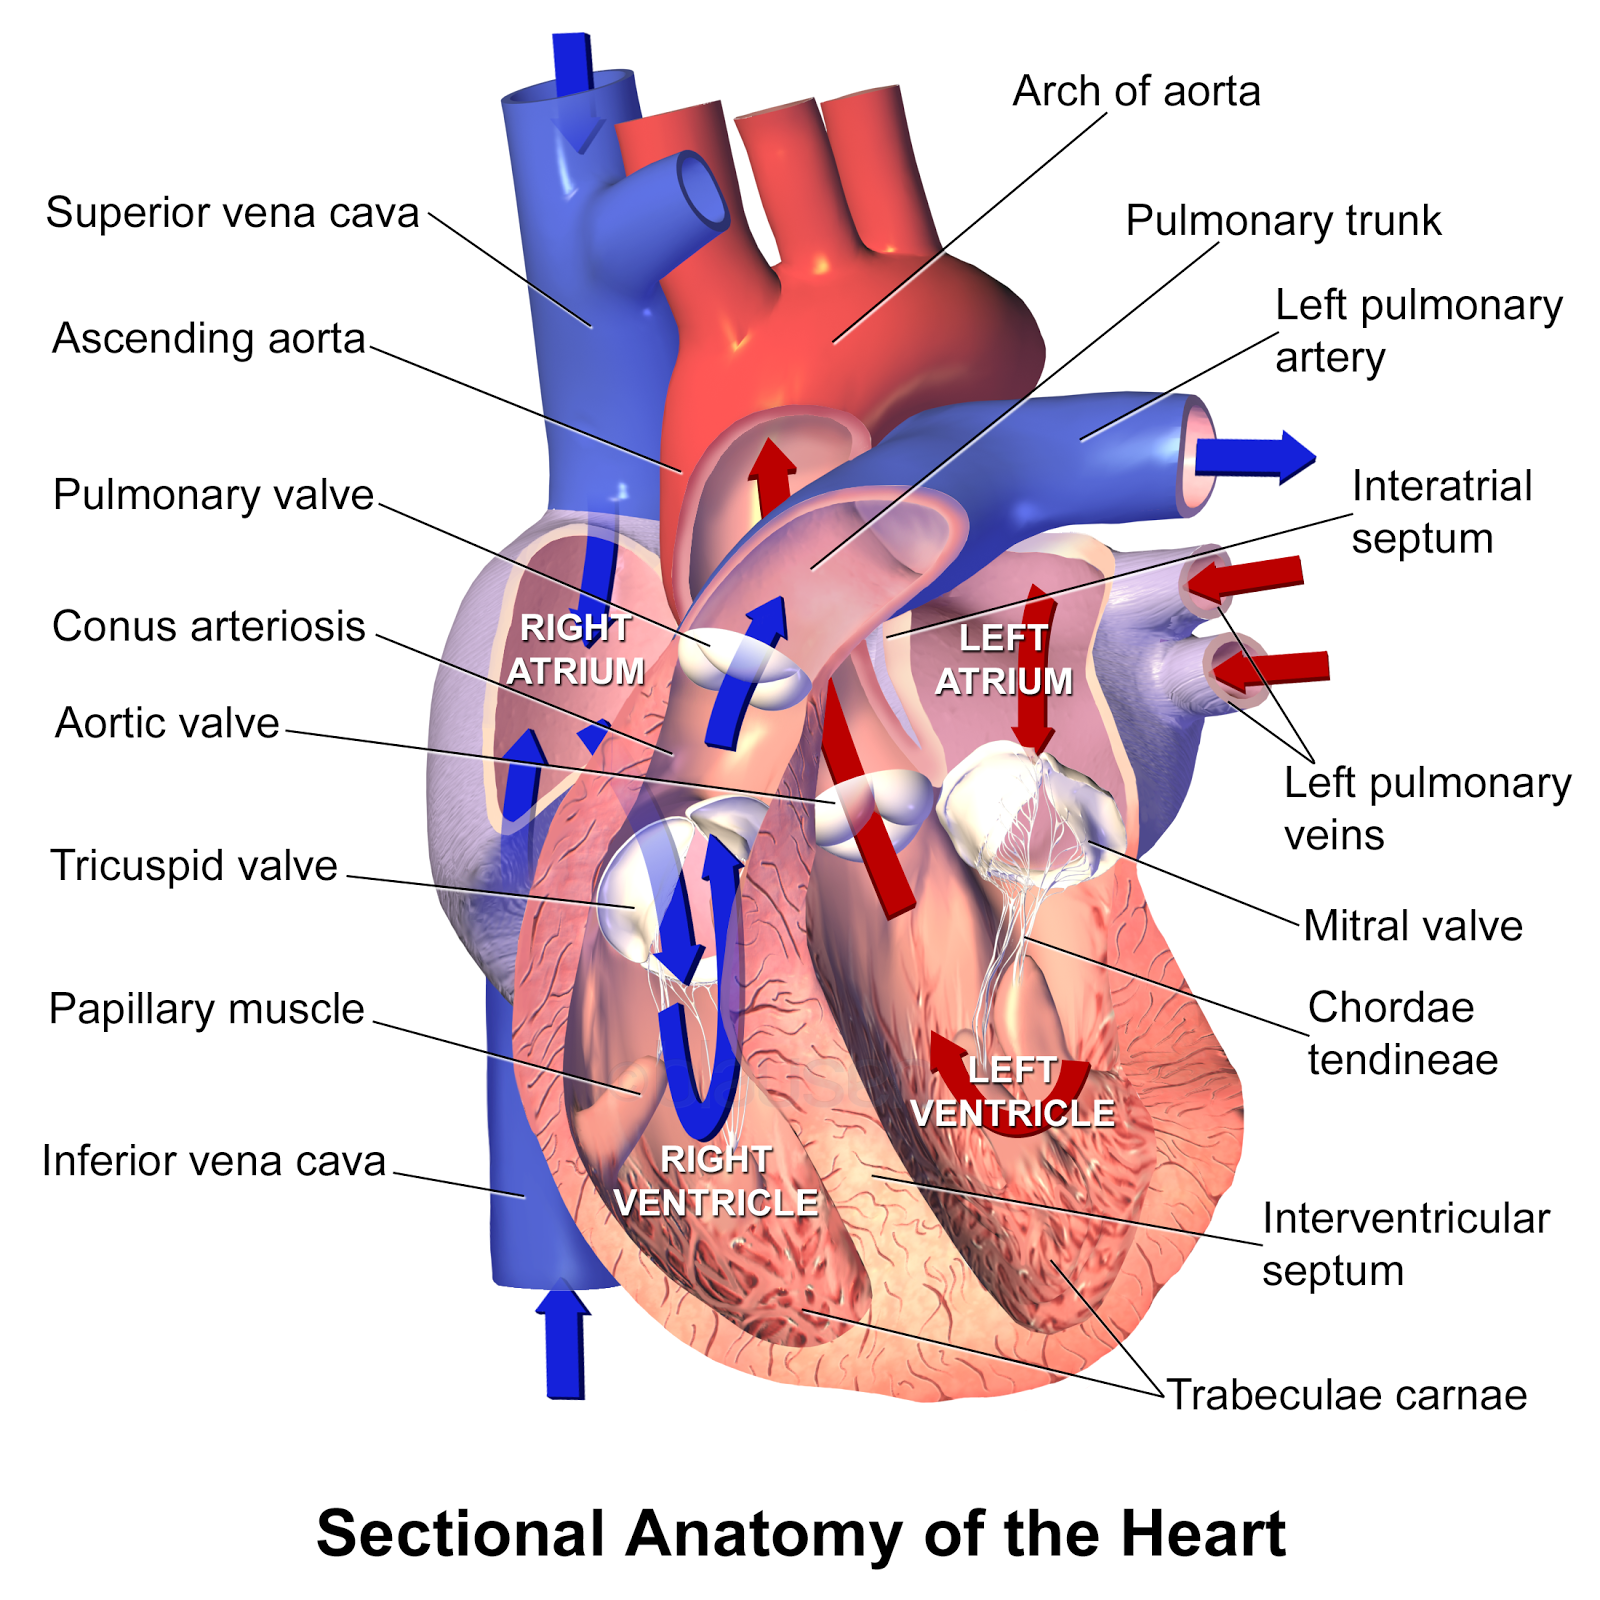
\includegraphics[width=100mm]{figures/ch2/human_heart_structure.png}
\caption{The human heart structure \label{overflow}}
\label{fig1.1}
\end{figure}